\subsection{Ensemble Toolkit}\label{ssec:entk}

An ensemble-based application is a \textbf{workflow}, i.e. tasks
with dependencies that determine the order of their execution. Subsets of
these tasks can be \textbf{workloads}, i.e., tasks whose dependencies have
been satisfied at a particular time and may be executed concurrently.
Ensemble-based application vary in the type of coupling between tasks, the
frequency and volume of information exchanged between these tasks, and the
executable of each task. This type of applications requires specific
coordination, orchestration and execution protocols, posing both
domain-specific and engineering challenges.

Ensemble Toolkit (EnTK), the topmost layer of RCT, simplifies the process of
creating and executing ensemble-based applications with complex coordination
and communication requirements. EnTK decouples the description of
ensemble-based applications from their execution by separating three orders
of concern: specification of task and resource requirements; resource
selection and acquisition; and task execution management. Domain scientists
retain full control of the implementation of their algorithms, programming
ensemble-based applications by describing what, when and where should be
executed. EnTK uses a runtime system, like RADICAL-Pilot, to acquire the
resources needed by applications to manage task execution.

EnTK enables the creation of ensemble-based applications by exposing an API
with four components: \textbf{Application Manager}, \textbf{Pipeline},
\textbf{Stage} and \textbf{Task}. Users describe ensembles in terms of
pipelines, stages and tasks, (PST), and pass this description to an instance
of Application Manager, specifying what resource to use for executing the
application (see Figure~\ref{fig:entk_arch}).

\begin{figure}
  \centering
  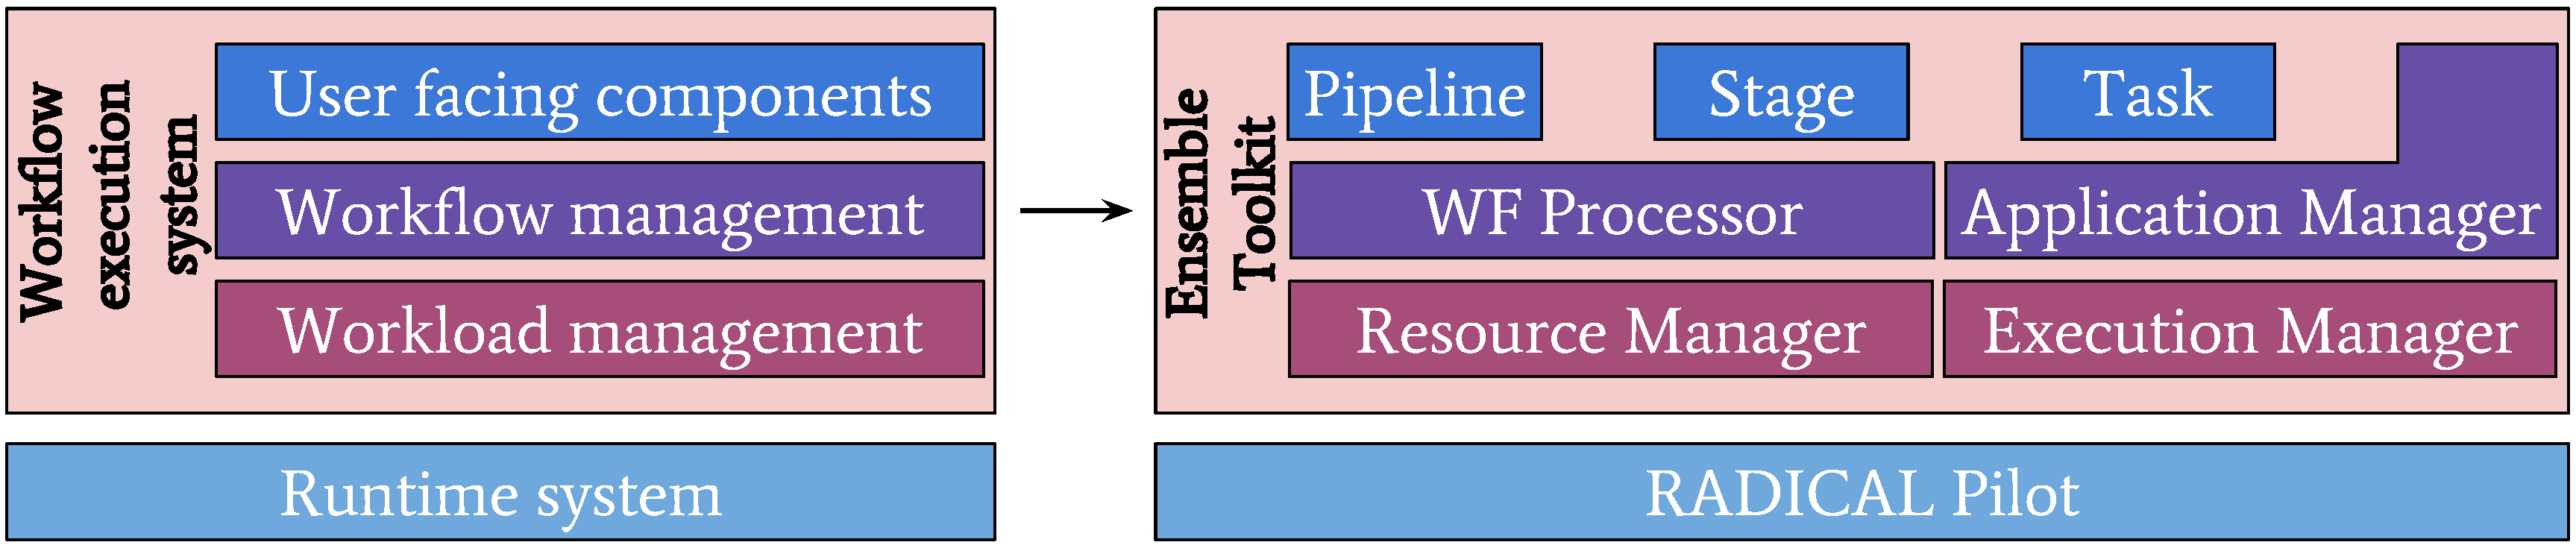
\includegraphics[width=\columnwidth]{FIGURES/entk_overview.pdf}
  \caption{\textbf{Left:} Ensemble Toolkit overview, showing how the abstract
           workflow execution system is mapped to specific components exposed
           to the users and components internal to the
           toolkit.}\label{fig:entk_arch}
\end{figure}

The Task component is used to encapsulate an executable and its software
environment and data dependencies. The Stage component contains a set of
tasks without mutual dependencies and that can therefore be executed
concurrently. The Pipeline component is used to describe a sequence of
stages, i.e., sets of tasks that need to be executed sequentially, not
concurrently.

The use of the Task, Stage, and Pipeline components, implemented as set and
list data structures, avoids the need to express explicitly relationship
among tasks. These relationships are insured by design, depending on the
formal properties of the lists and sets used to partition tasks into stages
and group stages into pipelines. Further, EnTK enables an explicit definition
of pre and post conditions on the execution of tasks, enabling a fine grained
adaptivity, both a local and global level. Conveniently, this does not
require the codification of a directed acyclic graph (DAG), a process that
imposes a rigid data-oriented \mtnote{data-oriented?} \jdnote{not sure what
you mean by data-oriented in this context} \jdnote{done} representation model
on the domain scientists~\cite{balasubramanian2017powerofmany}.

The \textbf{Application Manager} component of EnTK enables users to specify
target resources for the execution of the ensemble-based application. This
includes properties like walltime, number of nodes and credentials for
resource access. Users can also define execution setup parameters such as the
number of processes or messaging queues that should be used by EnTK\@. This
allows to size and tune the performance of EnTK, depending on the number of
tasks, stages and pipelines, but also on the resources available to the
toolkit.

The Application Manager along with the \textbf{WF Processor} is responsible
for the transformation of the application workflow into workloads, i.e., set
of tasks, that can be submitted to the indicated resources for execution.
Internally, the \textbf{Resource Manager} and \textbf{Execution Manager}
components enable the acquisition of resources and the management of
execution of these workloads (see \textbf{Figure~\ref{fig:entk_arch}}, right
schematic of left panel).